%% 信息一致评估（中文，与 main.tex 结构/论证对齐）
\documentclass[UTF8,a4paper,12pt]{ctexart}
\usepackage{amsmath,amssymb}
\usepackage{booktabs}
\usepackage{graphicx}
\usepackage{xurl}
\usepackage{microtype}
\usepackage{geometry}
\usepackage{setspace}
\usepackage[hidelinks]{hyperref}
\geometry{margin=2.54cm}
\onehalfspacing
\setlength{\emergencystretch}{2em}
\graphicspath{{figures/}{../ei_manuscript/figures/pub/}}

\title{锂离子电池剩余寿命的信息一致评估：\\
面向回顾性 oracle 的信息层级框架}
\author{江佳培\\
桂林电子科技大学商学院\\
\texttt{jjp@mails.guet.edu.cn}}
\date{}

\begin{document}
\maketitle

\begin{abstract}
\noindent
数据驱动的锂离子电池剩余寿命（RUL）预测通常以测试误差评估模型，却忽视了预测时刻的信息边界。
典型的信息泄漏源于相对寿命特征 $\mathrm{cycle\_norm}=t/T$ 与标签 $\mathrm{RUL}_t=T-t$ 共享目标寿命 $T$。
由于 $T$ 在预测阶段不可知，此类特征构成回顾性 oracle，有悖于在线部署的合法性。
为此，本文提出信息一致（information-consistent）评价协议，包含四个核心要素：嵌套信息层级（L0：原始 $t$；L1：留出目标后的群体先验 $t/T^{\mathrm{prior}}$；L1P：基于 SOH 匹配的同胞局部先验；L2：目标 oracle $t/T_{\mathrm{target}}$）、明确划分的拟合协议（同电芯回顾协议 A 与严格留出目标协议 B）、特征来源审计，以及结构化报告标准。
寿命终点定义为首次 SOH$\le 0.7$，未达标电芯作右删失处理。
MLP 与 Patch-TF 仅作为匹配的排序工具。
在 Severson 数据集（协议 B，$n{=}24$）上，MLP 的中位 RUL RMSE 从 L0 的 $222.1$ 显著降至 L2 的 $12.0$（Wilcoxon $p=1.2{\times}10^{-7}$），证实了信息层级对模型评估的决定性影响。
反直觉的是，在 NASA 协议 A 下，局部先验 L1P 的表现优于目标 oracle L2（如 B0005：$5.06$ vs.\ $23.58$）。
机理在于：L2 的时间时钟在测试窗中超出训练分布的支撑域（out-of-support），导致模型对晚寿命变化产生系统性高估；而 L1P 依赖于紧邻的 SOH 匹配距离，避免了时间外推风险。
该现象反映了模型的可学习性边界，并在协议 B 下得以反转（L1P $30.3$ vs.\ L2 $12.0$）。
本文的核心贡献在于建立一套可审计、可复现的 RUL 基准测试方法学标准，而非提出新的预测架构。
\end{abstract}

\noindent\textbf{关键词：}锂离子电池；RUL；信息可得性；评价协议；回顾性 oracle；留一电芯

\section{引言}
\label{sec:intro}

数据驱动的锂离子电池剩余寿命（RUL）预测在电池管理系统（BMS）中扮演核心角色~\cite{hu2019rser,xiong2018soh}。
近年来，深度序列模型（Transformer、Mamba、物理信息网络等）不断刷新固定特征集下的表观精度~\cite{lipu2018,wang2024gce,xu2025meas,yang2025batteries,zhang2025batlinet,deng2025piml,huang2025rulmamba,sun2026sgdits}。
然而，排行榜式评估往往忽略一个根本问题：在预测第 $t$ 个循环时，模型究竟被允许使用哪些信息？

一个普遍却常被忽视的信息泄漏，源于相对寿命特征的构造。
研究者通常将循环进度编码为
\begin{equation}
\mathrm{cycle\_norm}=\frac{t}{T},
\end{equation}
并以 $\mathrm{RUL}_t=T-t$ 作为监督标签。
由于定义标签的 $T$ 同时进入特征输入，模型实际上在回答回顾性问题；一旦去除该特征或改用固定时间尺度，许多先进模型的表观精度会大幅崩塌。
Geslin 等指出寿命特征必须与真实使用场景严格匹配~\cite{geslin2023joule}；近期 LOCO 与分组验证亦表明，不合时宜的同电芯随机划分或信息边界模糊会严重抬高表观精度~\cite{ali2026loco,barua2026predictor,madani2025groupkfold}。
在 NASA B0005 上，当把记录长度当作 $T$ 时，Patch-TF 的 RUL RMSE 由含该通道时的 $2.28\pm0.96$ 升至去掉后的 $18.83\pm3.88$~\cite{saha2007nasa}。

尽管机器学习领域对数据泄漏已有广泛讨论~\cite{kaufman2012leakage,kapoor2023leakage}，电池 RUL 评价仍存在三个具体缺口：
\begin{enumerate}
\item \textbf{缺乏可操作的嵌套信息层级。}
现有研究很少明确规定寿命端点常数 $T$ 在何种程度上被允许进入 $X_t$，也未能处理因 $T$ 定义不当导致的中间层级塌缩（如寿命同质数据中，群体先验与目标 oracle 重合）。
\item \textbf{信息层级与拟合协议混淆。}
大量研究将同电芯回顾性划分与留出跨电芯泛化混为一谈，忽略了标签构造与特征输入在信息合法性上的本质区别。
\item \textbf{基线不可复现与报告标准缺失。}
文献中通用的 Persistence 基线定义模糊，且缺少把信息层级、标准化来源、支撑域状态等审计字段与结果并列报告的结构化方式。
\end{enumerate}

因此，本文探讨的不是架构问题，而是评价协议的边界问题：模型的误差与排序，如何随预测时刻可用信息集 $\mathcal{I}_t$ 的变化而改变？
紧凑记法为
\begin{equation}
\boxed{\operatorname{Rank}(M_1,\ldots,M_k\mid \mathcal{I}_t)\;=\;f(\mathcal{I}_t).}
\end{equation}
为此，我们提出信息一致评估框架，将预测信息解构为四级循环通道：L0（原始 $t$）、L1（留出目标的群体先验 $t/T^{\mathrm{prior}}$）、L1P（基于 SOH 匹配的局部同胞诊断）与 L2（目标 oracle $t/T_{\mathrm{target}}$）；同时将拟合协议严格划分为同电芯回顾性协议 A 与严格留出目标的协议 B，并强制使用具名化的 Persistence 基线与右删失处理。
MLP 与 Patch-TF 仅作匹配排序仪器。

两项核心发现揭示了现有评价体系的脆弱性与机器学习的本质局限。
第一，在严格留出目标的 Severson 协议 B（$n{=}24$）中，MLP 的中位 RUL RMSE 从 L0 的 $222.1$ 骤降至 L2 的 $12.0$（Wilcoxon $p=1.2{\times}10^{-7}$），证实了目标寿命信息对排序的决定性影响。
第二，NASA 协议 A 上出现反直觉现象：信息更少的局部先验 L1P 居然优于拥有完整目标寿命的 oracle L2（如 B0005：$5.06$ vs.\ $23.58$）。
误差分解表明：按时间划分后，L2 的时间时钟在测试窗中偏离训练支撑域，网络压缩晚寿命变化并产生系统性高估；而 L1P 利用局部插值留在匹配邻域内。
更多信息如果``充分但不可学''，就无法转化为预测优势；该现象在协议 B 下反转（L1P $30.3$ vs.\ L2 $12.0$）。

\paragraph{贡献。}
（C1）\textbf{核心协议。}提出 L0/L1/L1P/L2 信息层级、首次 EOL 定义与右删失处理，分离协议 A/B，并提供包含通道支撑状态的逐输入来源审计表。\\
（C2）\textbf{机理发现。}精确解释``局部先验优于目标 oracle''的边界条件（分布外支撑、SOH 邻域覆盖），并给出其在不同协议下反转的证据。\\
（C3）\textbf{报告标准。}提出一行一条的模块化报告模板，使信息条件成为强制审计字段，为 BatteryML 等平台提供评测外壳~\cite{zhang2024batteryml}。\\
贡献是可审计、可复现的方法学标准，不是新的预测网络。

\section{相关工作}
\label{sec:related}

\paragraph{泄漏作为不合法的目标信息。}
Kaufman 等把泄漏定义为学习者不应合法获得的目标信息~\cite{kaufman2012leakage}。
Kapoor 与 Narayanan 记录了由此产生的不可复现排行~\cite{kapoor2023leakage}；行随机划分抬高性能并不限于电池~\cite{rosenblatt2024}。
电池 SOH/RUL 中，随机同电芯划分相对留出电芯（LOCO）也会抬高表观精度~\cite{barua2026predictor,ali2026loco}。
RUL 标签按定义必须使用未来 EOL；在在线主张下，不合法的是把该未来复制进 $X_t$。

\paragraph{BMS 监测、SOH 与 RUL。}
车载监测与状态估计是 BMS 的既有要求~\cite{hu2019rser}。
SOH 综述区分电化学诊断与数据驱动映射~\cite{xiong2018soh}。
RUL 综述覆盖滤波、神经网络与混合方法~\cite{lipu2018,wang2024gce,xu2025meas,yang2025batteries}，却往往未把循环时钟写进评价协议。
容量再生与混合老化会打破恒定衰减假设~\cite{birkl2017,aliakbari2025fusedr,fan2026meas}。

\paragraph{数据驱动 RUL 学习器与近期基准。}
经典预后基线仍是参照~\cite{saha2009compare}。
近期工作涵盖跨电芯深度学习~\cite{zhang2025batlinet}、物理信息早期预测~\cite{deng2025piml,oyewole2025uq}，以及 Transformer、Mamba 与双路径状态空间等序列模型~\cite{vaswani2017,nie2023patchtst,huang2025rulmamba,li2026dpmamba,sun2026sgdits}。
同类 RUL 序列与融合框架还包括~\cite{yi2025jps,tian2025energy,ge2025koopman,li2025adapt,wang2025jes}。
BatteryML 与 BatteryLife 等平台表明，仅有架构表并不能固定评价体制~\cite{zhang2024batteryml,tan2025batterylife,li2024lifetime}。
MC-Dropout 仅作附录 UQ 对照~\cite{gal2016}。
本文只用匹配的 Patch-TF 与 MLP 在受控 $\mathcal{I}_t$ 下作排序仪器，不作架构声明。

\paragraph{寿命数据、特征与评价协议。}
公开语料包括 NASA PCoE~\cite{saha2007nasa,saha2009compare}、CALCE~\cite{he2011calce}与 MIT/Stanford~\cite{severson2019nature}；多条件与终身数据仍在扩展~\cite{li2024lifetime,tan2025batterylife,zhang2025batlinet}。
Geslin 等表明特征合法性取决于使用场景~\cite{geslin2023joule}；现场数据带来额外可得性约束~\cite{sulzer2021joule}。
主张跨电芯泛化时，分组验证与 LOCO 日益被推荐~\cite{roman2021,madani2025groupkfold,ali2026loco,barua2026predictor}。
本文的 L2 通道 $t/T_{\mathrm{target}}$ 是回顾性相对寿命时钟：对完成寿命研究有信息量，但在在线合法主张下信息不一致。
本文缺口是可操作的 L0/L1/L1P/L2 阶梯、具名拟合协议与可填报告行。

\section{信息一致协议}
\label{sec:protocol}

\subsection{观测集与寿命}
\label{sec:Ot}

预测在完成第 $t$ 次放电之后进行。
容量 $Q_t$ 由放电电流积分得到；SOH 为该电芯 $Q_t/Q_1$。
EOL 阈值全程为 0.7。
\begin{equation}
T \;=\;
\begin{cases}
\min\{ \tau: \mathrm{SOH}_\tau \le 0.7\}, & \text{若集合非空},\\
T_{\mathrm{record}}, & \text{否则（右删失）},
\end{cases}
\end{equation}
并令
\begin{equation}
\label{eq:rul}
\mathrm{RUL}_t \;=\; \max(0,\, T-t).
\end{equation}
首次穿越之后的容量再生不再打开指向更晚穿越的正 RUL；$T$ 与~\eqref{eq:rul} 只用一个全局首次 EOL。
若用记录末循环代替 $T$，NASA B0005--B0007 看起来寿命相同（记录长度 168），但 EOL 实为 161、106、167（表~\ref{tab:life}）。

从未越过阈值的电芯具有\emph{删失}寿命：此时 $T$ 是观测终点，$\mathrm{RUL}_t$ 指向记录终点而非失效事件。
本文在表~\ref{tab:life} 中显式标注该情形：删失电芯的绝对 RUL 误差不可与真实失效电芯直接比较，尽管各信息层级共享同一标签，其\emph{排序}仍在内部有效。
本研究中 B0007 是唯一删失电芯（末值 SOH 约 0.76），其作用在第~\ref{sec:b0007} 节讨论。


观测集 $\mathcal{O}_t$ 可含
$\{Q_\tau,\overline{V}_\tau,\overline{I}_\tau,\overline{T}_\tau,\mathrm{std}(V)_\tau\}_{\tau\le t}$
（NASA；CALCE 仅有 SOH 与 $t$）、原始下标 $t$，以及仅在同电芯训练时段（或留出目标同胞）上拟合的标准化。
排除 $T_{\mathrm{target}}$、$t/T_{\mathrm{target}}$ 及任何需要完整目标轨迹的变换，下文具名的 L2 有意 oracle 条件除外。

在线合法输入的硬规则：
\begin{equation}
\boxed{T\in Y,\qquad T\notin X_t,\qquad X_t\subseteq\mathcal{O}_t.}
\end{equation}
L2 有意违反 $T\notin X_t$；该违反本身即被测量的 oracle 条件，不是未命名的协议错误。

\subsection{层级 L0 / L1 / L2 与诊断通道 L1P}
\label{sec:levels}

仅循环通道 $c_t$ 改变；其余输入通道固定。
嵌套对象是构造 $c_t$ 时\emph{允许的寿命常数}，而不是声称目标轨迹的预测时刻观测量构成严格信息滤子：
\begin{equation}
\label{eq:nested}
\begin{aligned}
\mathcal{K}_0&=\emptyset,&
\mathcal{K}_1&=\{T^{\mathrm{prior}}\},&
\mathcal{K}_2&=\{T^{\mathrm{prior}},T_{\mathrm{target}}\},\\
&\mathcal{K}_0\subset\mathcal{K}_1\subset\mathcal{K}_2,\\
c_t^{(0)}&=t,&
c_t^{(1)}&=\frac{t}{T^{\mathrm{prior}}},&
c_t^{(2)}&=\frac{t}{T_{\mathrm{target}}}.
\end{aligned}
\end{equation}
记 $\mathcal{I}_k$ 为使用通道 $c_t^{(k)}$ 的评价条件。
其中 $T^{\mathrm{prior}}=\mathrm{median}\{T_i:i\in D_{\mathrm{train}}\}$ 只用留出目标后的训练电芯；禁止 $\mathrm{median}(T_{\mathrm{all}})$。
L2 是\emph{有意 oracle}：目标完成寿命按构造进入 $X_t$。
仅当主张在线合法（$t$ 时刻不可得 $T_{\mathrm{target}}$）时，才把同一通道称为信息不一致；该在线读法只在 BMS 在线场景下写出。
因 $T^{\mathrm{prior}}$、$T_{\mathrm{target}}$ 对 $t$ 为常数，
\begin{equation}
\label{eq:affine}
c_t^{(1)}=\alpha\,c_t^{(0)},\qquad
c_t^{(2)}=\beta\,c_t^{(0)},\qquad
\alpha=(T^{\mathrm{prior}})^{-1},\ \beta=T_{\mathrm{target}}^{-1},
\end{equation}
故 L0/L1/L2 在\emph{输入}层面是同一下标 $t$ 的相互仿射（严格单调）变换。
嵌套 $\mathcal{K}_0\subset\mathcal{K}_1\subset\mathcal{K}_2$ 记录表征中允许的外部寿命常数，并不声称它们是目标预测时刻观测量的严格富集。
式~\eqref{eq:affine} \emph{不}蕴含网络输出不变性：训练后的 MLP/Patch-TF 不必满足 $\hat y^{(1)}=\hat y^{(2)}$。
协议 A 上 L1$\approx$L2 因此是经验尺度稳健性观察（第~\ref{sec:controls} 节），不是模型不变性定理，也不是学到了群体寿命尺度。

\begin{table}[htbp]
\centering
\footnotesize
\caption{仿射恒等式与经验误差相等不是同一命题：式~\eqref{eq:affine} 证明了什么、没有证明什么，以及区分二者的观察。}
\label{tab:affine}
\setlength{\tabcolsep}{4pt}
\begin{tabular}{@{}p{0.28\linewidth}p{0.17\linewidth}p{0.47\linewidth}@{}}
\toprule
命题 & 状态 & 证据 / 说明 \\
\midrule
$c^{(1)}=\alpha c^{(0)}$，$c^{(2)}=\beta c^{(0)}$，$\alpha,\beta>0$ & 已证 & 式~\eqref{eq:affine}；对 $t$ 严格单调 \\
L0/L1/L2 保持循环次序 & 蕴含 & 同一下标的单调变换 \\
训练后满足 $\hat y^{(1)}=\hat y^{(2)}$ & 不蕴含 & 协议 A 下平均 $|\hat y^{L1}-\hat y^{L2}|=0.02$--$0.25$ 循环（$\rho>0.97$）；协议 B 下 L1 $33.5$ vs.\ L2 $12.0$ \\
RUL RMSE 对重标度不变 & 不蕴含 & 协议 A：$23.62$ vs.\ $23.58$；时钟 $t/1000$：$23.11$；原始 $t$：$14.92$（B0005） \\
L1P 对 $t$ 仿射 & 按构造为假 & SOH 索引查表，式~\eqref{eq:l1p}；$\rho(\mathrm{L1P},\mathrm{L2})$ 在 $-0.12$ 到 $-0.82$ \\
\bottomrule
\end{tabular}
\end{table}

另设诊断通道
\begin{equation}
\label{eq:l1p}
\mathrm{L1P}_t \;=\; \mathrm{median}\bigl\{\mathrm{RUL}_{\tau_i}^{(i)}:\, i\in D_{\mathrm{train}},\;
\tau_i=\arg\min_{\tau}|\mathrm{SOH}_\tau^{(i)}-\mathrm{SOH}_t^{\mathrm{target}}|\bigr\}
\end{equation}
为：在目标已观测 SOH 处，取同胞上最近 SOH 点的剩余寿命中位数。
匹配前将目标 SOH 轨迹截断到 $t$；不用 $\mathrm{SOH}_{>t}^{\mathrm{target}}$ 与 $T_{\mathrm{target}}$。
L1P 与 L1 共用 $D_{\mathrm{train}}$，但\emph{不是}嵌套链~\eqref{eq:nested} 的元素：它是非仿射群体 RUL 映射，记为 L1P 而非 $\mathcal{K}_{1\mathrm{P}}$。
匹配质量用最近同胞循环处的绝对 SOH 距离报告（第~\ref{sec:controls} 节）。

首次 EOL 及之后 RUL$=0$ 的窗口在时序划分前删除，避免测试 RMSE 被全零尾部主导。

\subsection{协议 A/B 决策指引}
\label{sec:decision}

信息层级与拟合协议是两条独立轴；协议应由主张与可用数据决定，而不是由便利决定。
主张留出目标泛化、或寿命异质使绝对 $t$ 跨电芯不可比时，默认用协议 B（Severson 主证据）。
没有同胞池时，协议 A 是唯一可行选择；主张固定实验协议下的同电芯回顾倒计时时，它也是正当选择，但不能作为跨电芯信息层级的证据。
表~\ref{tab:decision} 把选择操作化。
两条推论：其一，若电芯没有同胞，L1 与 L1P 根本无法构造（既无 $T^{\mathrm{prior}}$，也无 SOH--RUL 图），单电芯研究只能比较 L0 与具名 L2 oracle，不能把 L0/L1/L2 排成信息层级；其二，若目标电芯没有早期历史（机队中的新电芯），协议 A 不可能，只有协议 B 有意义。
两者都可行时应同时报告；二者不一致本身就是协议敏感性的发现，不应取平均抹平。

\begin{table}[htbp]
\centering
\small
\caption{按主张与数据选择协议。“可构造层级”指实际可构造的层级；“可主张范围”是该设计支持的最强陈述。}
\label{tab:decision}
\begin{tabular}{@{}p{0.24\linewidth}p{0.18\linewidth}p{0.20\linewidth}p{0.30\linewidth}@{}}
\toprule
数据情形 & 可行协议 & 可构造层级 & 可主张范围 \\
\midrule
单电芯、无同胞 & 仅 A & L0、L2（oracle）；L1/L1P 不可定义 & 同电芯回顾倒计时；不作层级或跨电芯排序 \\
多电芯、寿命同质 & A（B 可行但退化） & L0、L2；L1$\approx$L2 & 同电芯诊断；B 因 $T^{\mathrm{prior}}\approx T_{\mathrm{target}}$ 增益很小 \\
多电芯、异质、目标有历史 & A 与 B & 四级 & 排序优先用 B；A 作协议敏感性对照 \\
多电芯、新目标、无历史 & 仅 B & L0、L1、L1P、L2 & 留出目标泛化；L1P 要求与同胞 SOH 重叠 \\
机队加目标历史、在线主张 & A 与 B & L0、L1、L1P（L2 具名 oracle） & 仅当 $T_{\mathrm{target}}\notin X_t$ 时在线合法 \\
\bottomrule
\end{tabular}
\end{table}

\subsection{拟合协议}
\label{sec:fit}

信息层级 $\mathcal{I}_t$ 与拟合协议是两条独立轴。
\begin{description}
\item[协议 A（同电芯回顾评价）。]
目标电芯预 EOL 窗口按循环时序划分：前 80\% 为支撑集，后 20\% 留作测试。
在前 80\% 支撑集内，仍按时序将末尾 15\% 窗口作验证、其余 85\% 作参数更新。
特征标准化 / $z(t)$ 仅在训练划分上拟合；验证与测试窗不参与标准化或参数估计；早停取验证集 RUL RMSE 最低检查点。
$W{=}50$ 滑动窗在时间上仍重叠，时序验证减轻但不消除 train/val 依赖；本文不声称窗口 i.i.d.\ 抽样。
即便 L0/L1 下 $T\notin X_t$，早期窗口标签 $\mathrm{RUL}_t=T_{\mathrm{target}}-t$ 仍编码该电芯寿命。
NASA 与 CALCE 用协议 A；Severson 协议 A 仅作同窗对照。
\item[协议 B（严格留出目标证据）。]
目标电芯样本不进入拟合、验证、标准化与 L1/L1P 构造；测试窗仍为同一后 20\%。
同胞池经种子固定置换后，末尾 15\% 作验证、其余作训练（早停同协议 A）。
Severson 主证据（表~\ref{tab:severson}）用协议 B。
代码：\path{scripts/run_info_levels_v2.py} 中 \texttt{--fit-protocol leave\_target}。
\end{description}

\subsection{Persistence}
\label{sec:persist}

具名报告 RUL 基线；未命名的``persistence''不可复现。
\begin{itemize}
\item \textbf{persist\_fade}（强制 L0 对照）：窗口首末 SOH 定衰减率，外推到 SOH$=0.7$；只用 $X_t\subseteq\mathcal{O}_t$。
\item \textbf{linear}：窗口内 SOH 对局部循环下标的最小二乘（亦为 L0 合法）。
\item \textbf{persist\_recursive}：$\widehat{\mathrm{RUL}}_t=\max(\widehat{\mathrm{RUL}}_{t-1}-1,0)$，由最后训练窗的 persist\_fade 初始化；不用真 RUL 标签。
\item \textbf{persist\_hold}（oracle 诊断）：$\widehat{\mathrm{RUL}}_t=\mathrm{RUL}_{t-1}$，使用上一时刻真标签。预测时 BMS 观测不到 $T-t$；该走步不是 L0 基线。
\end{itemize}

\subsection{来源审计}
\label{sec:audit}

表~\ref{tab:provenance} 为信息流矩阵。
标签可依赖 $T$；输入不可。
$I(\mathrm{error};T)>0$ 不作``不合法 oracle''证明：短寿命电芯在 L0 下可以本身更难。

\begin{table}[htbp]
\centering
\caption{信息流审计。标签可用 $T$；输入不可。L1 统计只来自 $D_{\mathrm{train}}$。}
\label{tab:provenance}
\begin{tabular}{@{}p{0.28\linewidth}p{0.22\linewidth}p{0.22\linewidth}p{0.22\linewidth}@{}}
\toprule
流水线阶段 & L0 & L1 / L1P & L2 \\
\midrule
原始观测 & $\tau\le t$ & 同左 & 允许完整目标轨迹 \\
目标寿命 $T$ & 禁止 & 禁止 & 允许 \\
标签构造 & $T$ 仅在 $Y$ & 同左 & 同左 \\
目标归一化 $t/T$ & 禁止 & 禁止 & 允许 \\
训练电芯 $T^{\mathrm{prior}}$ / SOH--RUL 图 & 禁止 & 允许（非目标） & 允许 \\
训练 scaler / $z(t)$ & 仅训练期 & 仅训练期 & 仅训练期 \\
测试集统计量 & 禁止 & 禁止 & oracle 运行中允许 \\
VMD/EMD & 仅因果 & 仅因果 & 允许全轨迹 \\
窗口 & 仅过去 & 仅过去 & 此处仅过去 \\
超参 / 特征选择 & 仅训/验 & 同左 & 同左 \\
\bottomrule
\end{tabular}
\end{table}

\subsection{报告模板}
\label{sec:template}

每条实验一行
（模型、语料、电芯、层级、循环通道公式、$W$，$H$、scaler 来源、RUL RMSE、persist\_fade RMSE、可选 SOH RMSE）。
附录表~\ref{tab:template} 为可填表。
RUL 表最低要求：L0 与 persist\_fade，以及明确的 $T$ 定义。

\section{实验设置}
\label{sec:setup}

\paragraph{数据与角色。}
NASA PCoE B0005--B0007~\cite{saha2007nasa} 为协议 A 下的诊断语料：相同 2\,Ah 协议、共享记录长度、异质 EOL，以及同电芯时序倒计时。
CALCE CS2\_35--38~\cite{he2011calce} 为协议 A 跨语料复现（EOL 为 $\{349,418,410,388\}$；本地提取仅 SOH 与循环通道）。
MIT/Stanford Severson~\cite{severson2019nature} 为协议 B 下的主异质寿命应力检验，协议 A 作同窗对照。
Braatz 剔除后，119 电芯到达公开 80\% 标称 EOL（$T$ 由 QDischarge$/1.1\le 0.8$）。
评分子集事先固定为分层应力设计 $n{=}24{=}8{+}8{+}8$：按 $T$ 排序，取最短 8、最长 8、中位附近连续 8（不是对 119 的总体估计）。
电芯名单与 $T$ 见 \path{outputs/info_levels_severson/selection.json}。
每颗在协议 B（表~\ref{tab:severson}）与协议 A 同测试窗（表~\ref{tab:severson_A}）下跑完 L0/L1/L1P/L2。
$T^{\mathrm{prior}}$ 与 L1P 用留出目标后的 119 池，禁止 $\mathrm{median}(T_{\mathrm{all}})$。
协议 B 下，评分目标也不进入模型拟合与 L1/L1P 构造。
NASA/CALCE 的 $T$ 仍为 SOH$\le 0.7$。

\paragraph{模型。}
MLP 与 Patch-TF（匹配双 SOH/RUL 头、软物理约束，$d{=}64$，两层，$W{=}50$，$H{=}5$，种子 $\{42,43,44\}$，80 epoch，验证 RUL RMSE 早停）。
Patch-TF 沿用 patch 序列 Transformer~\cite{vaswani2017,nie2023patchtst}，不是新骨干。
\textbf{默认双头目标}为尺度平衡损失 $\mathcal{L}_{\mathrm{SOH}}+0.5\,\mathcal{L}_{\mathrm{RUL}/T}$（RUL 目标除以 $T$，评估时再乘回 $T$），使两头同为 $O(1)$，避免原始循环尺度的 RUL 项饿死 SOH 头。
阶梯排序表同时保留未归一化历史目标 $\mathcal{L}_{\mathrm{SOH}}+0.5\,\mathcal{L}_{\mathrm{RUL}}$ 作为消融；第~\ref{sec:controls} 节表明，在健康默认配置下信息层级排序不变。
修订实验在 CPU 上完成；排序声明不依赖特定 GPU。

\paragraph{指标。}
头条为 RUL RMSE（循环数）。
同窗 SOH RMSE 为辅助对照：循环通道是否变成静默 SOH oracle。
MC-Dropout 的 PICP/PINAW 仅附录~\cite{gal2016}；不作校准声明。

\paragraph{统计。}
每颗电芯、每个模型的种子级 RMSE（$n{=}3$）为技术重复。
排序翻转声明的独立单元是电芯：$e_i=\mathrm{RMSE}_{L0,i}-\mathrm{RMSE}_{L2,i}$，跨电芯配对 Wilcoxon。
该检验比较 L0 与 L2 误差是否不同；本身不决定使用场景合法性。
NASA+CALCE 用 $n{=}7$；Severson 用分层 $n{=}24$。

\section{结果}
\label{sec:results}

结果分三层报告。
主证据：Severson 协议 B（$n{=}24$）上，MLP 中位 RUL RMSE 由 L0 的 $222.1$ 降至 L1 $33.5$、L1P $30.3$、L2 $12.0$，且所评电芯上 L0 均高于 L2（图~\ref{fig:seversonb}）。
次级：NASA 协议 A 上 L1P 可优于 L2（图~\ref{fig:l1pnasa}），说明更多目标寿命信息未必降低测试误差。
诊断：协议 A 上 L1$\approx$L2 对应输入仿射加经验尺度稳健性；同电芯晚寿命倒计时下，原始 $t$ 也可优于 L2。
NASA/CALCE（$n{=}7$）为探索；CALCE 与 MC-Dropout 降级。

\subsection{用 EOL 定义 $T$ 才能分开 L1}
\label{sec:life}

表~\ref{tab:life} 与图~\ref{fig:soh} 给出结构修正。
NASA 记录长度相同，EOL 不同。
B0005 的 L1 分母为 $\mathrm{median}(106,167)=136.5$，目标 $T=161$；
B0006 为 164 对 106；B0007 为 133.5 对 167。
L1 因此不再是 L2 的拷贝。
CALCE 同胞中位数同样不等于各目标（如 CS2\_35：$T=349$，同胞中位数 $410$）。

\begin{table}[htbp]
\centering
\caption{寿命定义。$T_{\mathrm{record}}$ 为最后放电下标；$T_{\mathrm{EOL}}$ 为首次 SOH$\le 0.7$。再生量为 SOH 正增量之和。“达到 EOL”为“否”时，$T$ 是右删失时间（最后观测循环）。}
\label{tab:life}
\begin{tabular}{@{}llrrrrr@{}}
\toprule
语料 & 电芯 & $n$ & $T_{\mathrm{record}}$ & $T_{\mathrm{EOL}}$ & 再生量 & 达到 EOL \\
\midrule
NASA & B0005 & 168 & 167 & 161 & 0.222 & 是 \\
NASA & B0006 & 168 & 167 & 106 & 0.367 & 是 \\
NASA & B0007 & 168 & 167 & 167 & 0.182 & 否（删失） \\
CALCE & CS2\_35 & 882 & 881 & 349 & 1.665 & 是 \\
CALCE & CS2\_36 & 936 & 935 & 418 & 1.929 & 是 \\
CALCE & CS2\_37 & 972 & 971 & 410 & 2.011 & 是 \\
CALCE & CS2\_38 & 996 & 995 & 388 & 2.341 & 是 \\
\bottomrule
\end{tabular}
\end{table}

\begin{figure}[htbp]
\centering
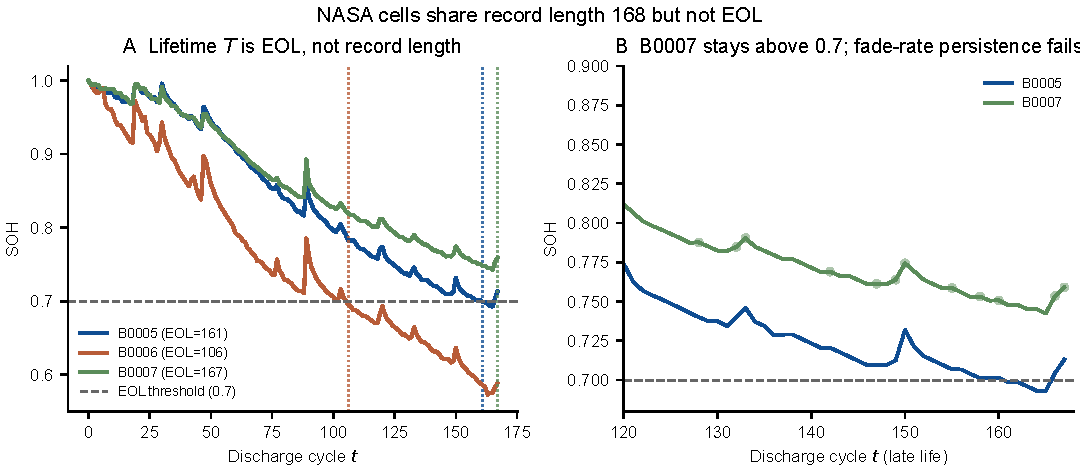
\includegraphics[width=0.98\linewidth]{fig_soh_trajectories.pdf}
\caption{NASA SOH--循环。
（A）记录长度均为 168，竖虚线为 $T_{\mathrm{EOL}}$。
（B）B0007 晚寿命仍高于 0.7，且常有向上跳动，恒定衰减 persistence 会给出过大剩余寿命。}
\label{fig:soh}
\end{figure}

\subsection{Severson 协议 B（主证据）}
\label{sec:severson}

本小节为主证据。
在 Severson~\cite{severson2019nature} 上，以短/中/长分层子集（$n{=}24$；$T$ 从 147 到 1933）在两种拟合协议下用 MLP 评分；L1/L1P 来自全留出目标同胞池。
协议 B 为主证据（图~\ref{fig:seversonb}；表~\ref{tab:severson}）；协议 A 为同测试窗对照（表~\ref{tab:severson_A}）。
协议 B 跨电芯中位 RUL RMSE 为 L0 $222.1$、L1 $33.5$、L1P $30.3$、L2 $12.0$。
配对 Wilcoxon $p=1.2{\times}10^{-7}$；所评电芯上 L0 均高于 L2。
具名 L0 基线：persist\_fade 中位 $242.8$，persist\_recursive $499.4$；persist\_hold$=1.0$。
相对协议 A（L2/L1/L1P/L0 中位 $15.9$/$16.9$/$19.0$/$73.4$），去掉目标训练标签后 L0--L2 差距拉大。
协议 B 下输入仿射~\eqref{eq:affine} 不再给出 L1$\approx$L2；常数群体时钟无法在异质 $T$ 上恢复目标特异相对寿命。
L1P 仍为~\eqref{eq:nested} 外的非仿射诊断；其协议 B 中位误差（$30.3$）\emph{高于} L2（$12.0$），故下一节的反转是协议特异的。

\begin{figure}[htbp]
\centering
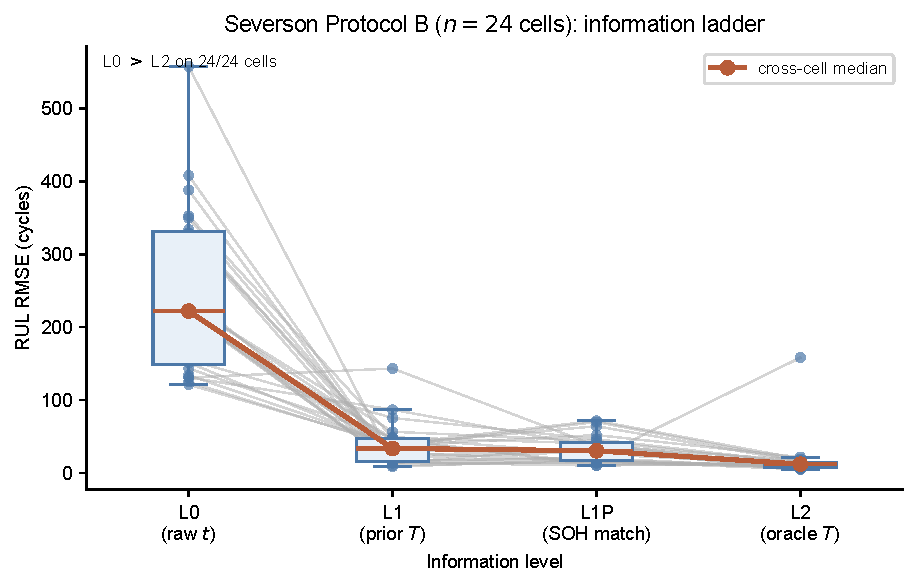
\includegraphics[width=0.98\linewidth]{fig_severson_protocol_b.pdf}
\caption{Severson 协议 B 信息阶梯（主证据；$n{=}24$）。
逐电芯 MLP 轨迹、箱线与跨电芯中位叠加。
中位：L0 $222.1$，L1 $33.5$，L1P $30.3$，L2 $12.0$。
所评电芯上 L0$>$L2（配对 Wilcoxon $p=1.2{\times}10^{-7}$）。}
\label{fig:seversonb}
\end{figure}

% auto-generated Severson Protocol A/B summary
\begin{table}[htbp]
\centering
\caption{Severson Protocol~A within-cell retrospective evaluation (chronological fit; MLP; stratified 24 cells; leave-target $T^{\mathrm{prior}}$ only). Cross-cell median RUL RMSE (cycles). Support comparison.}
\label{tab:severson_A}
\begin{tabular}{@{}lcccc@{}}
\toprule
Fit & L2 & L1 & L1P & L0 \\
\midrule
Protocol~A ($n=24$) & 15.9 & 16.9 & 19.0 & 73.4 \\
\bottomrule
\end{tabular}
\end{table}

\begin{table}[htbp]
\centering
\caption{Severson Protocol~B strict leave-target-cell-out evidence (MLP; same stratified 24 cells and same late-20\% test windows; train/val on sibling cells only; L1/L1P from the leave-target 119-cell pool). Cross-cell median RUL RMSE (cycles). Main evidence.}
\label{tab:severson}
\begin{tabular}{@{}lcccc@{}}
\toprule
Fit & L2 & L1 & L1P & L0 \\
\midrule
Protocol~B ($n=24$) & 12.0 & 33.5 & 30.3 & 222.1 \\
\bottomrule
\end{tabular}
\end{table}

\begin{table}[htbp]
\centering
\caption{Severson L0-valid classical foils on the same late-20\% test windows as Protocol~B ($n=24$). Cross-cell median RUL RMSE (cycles). persist\_hold $=1$ is an oracle label walk, not an L0 foil.}
\label{tab:severson_base}
\begin{tabular}{@{}lccc@{}}
\toprule
Baseline & persist\_fade & linear & persist\_recursive \\
\midrule
Protocol~B test windows & 242.8 & 228.2 & 499.4 \\
\bottomrule
\end{tabular}
\end{table}

% Protocol A Wilcoxon L0 vs L2: p=1.1920928955078125e-07, frac=1.00
% Protocol B Wilcoxon L0 vs L2: p=1.1920928955078125e-07, frac=1.00
% Protocol B classical medians: {'persist_fade': 242.77778588407944, 'linear': 228.2162851240011, 'persist_recursive': 499.3628845214844, 'persist_hold': 1.0, 'persist_mean': 299.36610154957066}
\begin{table}[htbp]
\centering
\footnotesize
\caption{Severson Protocol~B per-cell MLP RUL RMSE excerpt (mean over three seeds). Short / mid / long $T$ strata.}
\label{tab:severson_cells}
\begin{tabular}{@{}lcccc@{}}
\toprule
Cell & L2 & L1 & L1P & L0 \\
\midrule
b2c1 & 158.2 & 17.1 & 20.5 & 557.7 \\
b2c0 & 13.7 & 14.3 & 10.0 & 408.1 \\
b2c3 & 10.4 & 10.3 & 15.1 & 388.0 \\
b2c47 & 8.0 & 13.5 & 36.0 & 219.0 \\
b1c15 & 4.9 & 27.7 & 16.3 & 215.0 \\
b1c32 & 8.4 & 13.3 & 13.5 & 225.2 \\
b3c45 & 15.4 & 39.0 & 64.0 & 133.8 \\
b3c7 & 21.6 & 37.2 & 51.9 & 124.9 \\
b3c38 & 19.0 & 39.3 & 71.6 & 121.2 \\
\bottomrule
\end{tabular}
\end{table}


\subsection{L1P 为何能优于 L2：支撑而非信息}
\label{sec:mechanism}

表~\ref{tab:ladder} 与图~\ref{fig:l1pnasa} 给出反转：NASA 协议 A 上，MLP 的 L1P RMSE 为 $5.06\pm0.23$（B0005）、$5.45\pm0.45$（B0006）、$8.66\pm0.10$（B0007），对应 L2 为 $23.58\pm3.85$、$10.62\pm1.69$、$20.19\pm3.80$；Patch-TF 复现同一次序（B0005：$2.84$ vs.\ $19.17$）。
首先排除匹配失败：平均绝对 SOH 匹配距离仅 $0.0039$（B0005）、$0.0307$（B0006）、$0.0010$（B0007）。
其次排除“偷偷多用信息”：目标 SOH 轨迹在 $t$ 处截断，$T_{\mathrm{target}}$ 与未来 SOH 都不进入式~\eqref{eq:l1p}。
剩下的问题是：目标寿命信息\emph{更少}的通道，为何误差更低。

\paragraph{oracle 时钟充分但在此不可学。}
首次 EOL 标签下 $\mathrm{RUL}=T(1-c^{(2)})$，对 L2 通道做线性读出即可精确恢复 RUL；附录 OLS 检查在 NASA 与 CALCE 上对原始 $t$ 给出零误差。
信息是充分的，失效发生在拟合器。
协议 A 按时间划分窗口，故每个评分测试窗都有 $c^{(2)}>\max C_2$（第~\ref{sec:levels} 节）：网络在训练中从未见过时钟的晚寿命段。
在该支撑外区段，MLP 响应被压缩（预测标准差仅为真值标准差的 $0.42$--$0.50$），并把 RUL 高估 $10$--$23$ 个循环；超出训练上界每单位 $c^{(2)}$ 的有符号误差斜率约 $107$--$166$ 循环（表~\ref{tab:mechanism}、图~\ref{fig:mechanism}B）。
误差最大的位置恰是维护最关心的区段：$\mathrm{RUL}<10$ 时 L2 RMSE 达 $28$--$30$ 循环，而 L1P 为 $6$--$13$（图~\ref{fig:mechanism}C）。
所谓“更多信息没有帮助”，指的是信息在通道里存在，却落在学习器可用的区域之外。

\paragraph{局部先验是插值，残差也说明了这一点。}
L1P 以目标当前 SOH 索引，而不是以循环进度索引，因此即使循环时钟离开训练支撑，它的查表仍落在同胞 SOH 范围内。
测试窗上 L1P 平均高估 $4.4$--$7.9$ 循环，约为 L2 偏差的一半；其绝对误差与 SOH 匹配距离在评分窗上正相关（$r=0.75$、$0.76$、$0.27$）。
若把整条轨迹混在一起，相关会变成负的（$-0.53$、$-0.59$、$-0.10$），因为早期窗口同时具有很小的匹配距离和很大的绝对 RUL；条件在晚寿命评分窗上，符号才反转。
L1P 也不是通道值的简单拷贝：单独使用先验的 RMSE 为 $7.25$（B0005）、$3.26$（B0006）、$23.61$（B0007），拟合模型则为 $5.06$、$5.46$、$8.66$，说明共享主干用 SOH 轨迹对先验作了修正（在删失的 B0007 上最明显）。

\paragraph{边界条件。}
反转需要三者同时成立：（i）协议 A，使目标早期轨迹进入训练集；（ii）oracle 时钟的评分值落在训练支撑之外；（iii）同胞池的 SOH 范围覆盖目标晚寿命 SOH。
去掉任一条，反转即消失。
协议 B 下 L1P（$30.3$）差于 L2（$12.0$），因为群体先验无法在异质电芯上恢复目标特异寿命尺度。
CALCE 的 CS2\_36 又把 NASA 的次序反过来（L1P $60.69$ vs.\ L2 $2.20$），因为强再生下 CALCE 同胞的 SOH--RUL 关系并不局部稳定。
故 L1P 是局部群体结构的诊断，不是默认在线估计器。

\paragraph{对在线 BMS 的含义。}
$T$ 未知时，进度时钟根本不可用；在在线合法选项中，若存在可比机队且其 SOH 覆盖目标工作区间，SOH 索引的机队先验比未校准的循环进度外推更稳妥。
没有这样的机队时，仍应退回 L0 递归走步，并把 L2 oracle 仅作为回顾性上界报告。
这是使用场景陈述，不是“L1P 普遍优于 L2”的主张。

\begin{table}[htbp]
\centering
\small
\caption{L1P 反转的误差结构（NASA 协议 A；测试窗、三种子合并）。偏差为 $\mathrm{mean}(\hat y-y)$（循环）。“标准差比”为 L2 在评分窗上的 $\mathrm{s.d.}(\hat y)/\mathrm{s.d.}(y)$，小于 1 表示响应被压缩。末列为 L1P 的 SOH 匹配距离与其绝对误差在评分窗上的 Pearson 相关。}
\label{tab:mechanism}
\begin{tabular}{@{}lrrrrrr@{}}
\toprule
电芯 & L2 RMSE & L2 偏差 & L2 标准差比 & L1P RMSE & L1P 偏差 & $r(\mathrm{dist},|e|)$ \\
\midrule
B0005 & 23.79 & $+22.60$ & 0.50 & 5.06 & $+4.38$ & 0.75 \\
B0006 & 10.70 & $+10.01$ & 0.42 & 5.46 & $+5.18$ & 0.76 \\
B0007 & 20.43 & $+19.05$ & 0.50 & 8.66 & $+7.93$ & 0.27 \\
\bottomrule
\end{tabular}
\end{table}

\begin{figure}[htbp]
\centering
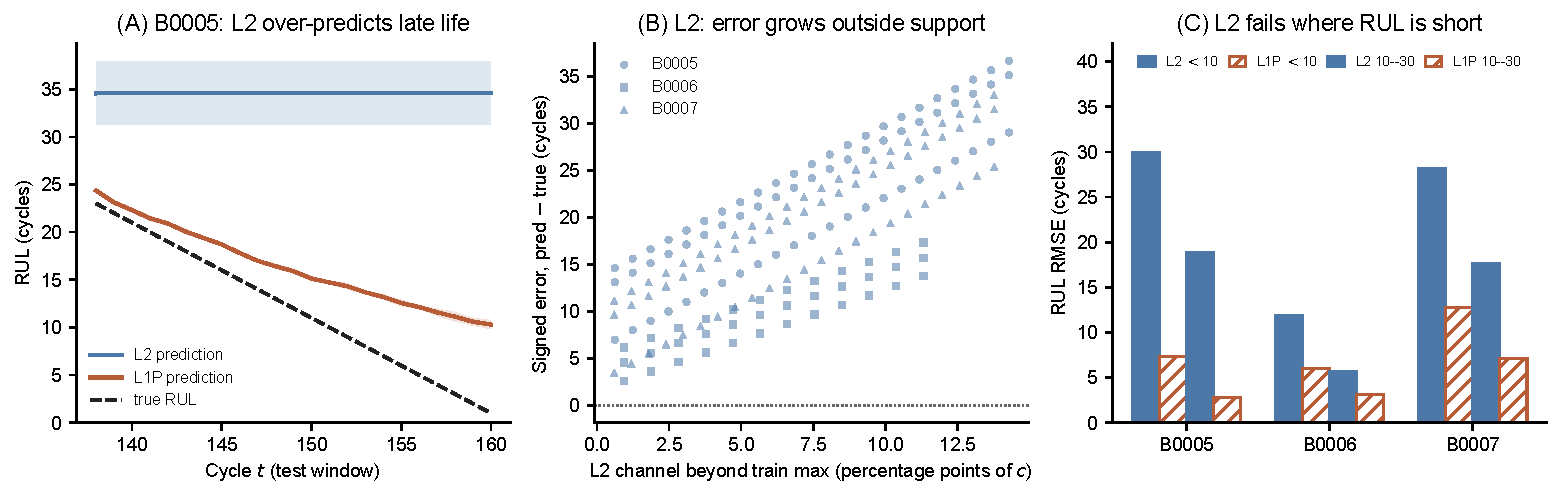
\includegraphics[width=0.99\linewidth]{fig_l1p_mechanism.pdf}
\caption{L1P 反转的机理（NASA 协议 A；MLP，三种子）。
（A）B0005 上 L2 预测几乎平在 $\sim 35$ 循环，而真实 RUL 已降到零；阴影为种子间 $\pm$1 标准差。
（B）三颗电芯的 L2 有符号误差都随评分通道值超出训练上界的距离增大。
（C）L2 误差在短 RUL 区最大，而这正是维护最关心的区段。}
\label{fig:mechanism}
\end{figure}

\subsection{信息阶梯上的重训}
\label{sec:ladder}

本小节展示排序如何随拟合协议移动；它\emph{不是}信息层级的证据，也不与 Severson 合并。
图~\ref{fig:ladder} 与表~\ref{tab:ladder} 给出 $T:=T_{\mathrm{EOL}}$、L0$=$原始 $t$、仅保留 RUL$>0$ 窗口、并纳入 B0006 的重训。
L1 与 L2 的\emph{分母}已经不同（表~\ref{tab:life}）；RMSE 不必呈同一阶梯。

协议 A 下，NASA 上 Patch-TF 的 L1 与 L2 误差到小数点后两位仍重合（如 B0005 均为 $19.17\pm2.42$）。
由~\eqref{eq:affine}，这是循环时钟的仿射等价，不是 $T^{\mathrm{prior}}$ 被当作学到的寿命尺度来用。
同电芯回顾划分上，原始 $t$ 的 L0 反而更容易（Patch-TF B0005 $10.21\pm1.21$；B0006 $4.63\pm0.33$；MLP 表~\ref{tab:ladder} B0005 L0 $11.77\pm0.15$ vs.\ L2 $23.58\pm3.85$）：测试段落在寿命后期，$\mathrm{RUL}\approx c-t$，未缩放的 $t$ 与标签同尺度。
第~\ref{sec:legacy} 节的 L0-drop 表明：\emph{去掉}循环通道会塌缩精度；改尺度不会。

因 $\mathrm{RUL}=T-t$，同窗 OLS 恒等式检查可从原始 $t$ 代数恢复 $T$；本文不把它当作预测基线（附录表~\ref{tab:clock}）。
L1P 打破与 L2 的仿射等价（$\rho(\mathrm{L1P},\mathrm{L2})$ 在 $-0.12$ 到 $-0.82$）。
对 B0005，$\mathrm{median}(T_{\mathrm{all}})=161=T_{\mathrm{target}}$ 而 $T^{\mathrm{prior}}=136.5$，若把测试电芯并入先验，L1 会按构造塌向 L2。

NASA 上 MLP 的 L1P RMSE 为 $5.06\pm0.23$（B0005）、$5.45\pm0.45$（B0006）、$8.66\pm0.10$（B0007）。
CALCE 上同一诊断不构成阶梯：CS2\_36 的 L1P 为 $60.69\pm20.40$，相对 L2 $2.20\pm1.30$ 与 L0 $40.33\pm2.14$（表~\ref{tab:ladder}）。
故 $\operatorname{Rank}_{L1P}$ 可与 $\operatorname{Rank}_{L2}$ 不同，而无须普遍的 $\mathrm{L2}\prec\mathrm{L1P}\prec\mathrm{L0}$。
首次 EOL 标签下，CS2\_35--38 上仿射 L1 贴近 L2，而原始 $t$ 的 L0 更难（如 CS2\_36：L1 $2.28\pm1.12$，L2 $2.20\pm1.30$，L0 $40.3\pm2.1$）。
CALCE 双通道上的 Patch-TF 不是可靠架构排名；只作匹配运行，不作胜出声明。

$n=3$ 种子的 Wilcoxon 检验（附录表~\ref{tab:stats}）仅作描述，不作推断。
七颗电芯上 MLP 的配对 Wilcoxon（$e_i=\mathrm{RMSE}_{L0,i}-\mathrm{RMSE}_{L2,i}$）$p=0.219$（表~\ref{tab:cellstat}）：NASA 上 L0 更容易，CALCE 上 L0 更难，故不存在单一的电芯总体阶梯。
主推断仍为 Severson 协议 B 的电芯级对比（第~\ref{sec:severson} 节）。

% auto-generated; do not edit by hand
\begin{table}[htbp]
\centering
\caption{Information ladder RUL RMSE (cycles; mean$\pm$s.d.\ over three seeds). $T$ is the EOL cycle (SOH$\le 0.7$). L0 uses raw $t$. L1 uses $t/T^{\mathrm{prior}}$ from leave-target training cells. L1P is MLP only: SOH-matched sibling RUL.}
\label{tab:ladder}
\begin{tabular}{@{}llcccc@{}}
\toprule
Model & Cell & L2 & L1 & L1P & L0 \\
\midrule
\multicolumn{6}{l}{\textit{NASA}} \\
mlp & B0005 & 23.58$\pm$3.85 & 23.62$\pm$3.89 & 5.06$\pm$0.23 & 11.77$\pm$0.15 \\
mlp & B0006 & 10.62$\pm$1.69 & 10.52$\pm$1.70 & 5.45$\pm$0.45 & 6.46$\pm$0.99 \\
mlp & B0007 & 20.19$\pm$3.80 & 20.16$\pm$3.70 & 8.66$\pm$0.10 & 11.22$\pm$2.68 \\
patch-tf & B0005 & 19.17$\pm$2.43 & 19.17$\pm$2.42 & 2.84$\pm$0.89 & 10.21$\pm$1.21 \\
patch-tf & B0006 & 10.11$\pm$0.23 & 10.11$\pm$0.23 & 3.10$\pm$0.19 & 4.63$\pm$0.33 \\
patch-tf & B0007 & 15.25$\pm$2.27 & 15.26$\pm$2.27 & 3.62$\pm$0.73 & 10.84$\pm$2.08 \\
\multicolumn{6}{l}{\textit{CALCE}} \\
mlp & CS2\_35 & 2.73$\pm$1.38 & 3.00$\pm$2.15 & 18.19$\pm$9.40 & 33.42$\pm$2.78 \\
mlp & CS2\_36 & 2.20$\pm$1.30 & 2.28$\pm$1.12 & 60.69$\pm$20.40 & 40.33$\pm$2.14 \\
mlp & CS2\_37 & 2.72$\pm$1.00 & 2.86$\pm$1.11 & 15.68$\pm$0.97 & 45.28$\pm$2.45 \\
mlp & CS2\_38 & 11.87$\pm$1.95 & 12.40$\pm$1.60 & 53.74$\pm$3.25 & 46.00$\pm$3.99 \\
patch-tf & CS2\_35 & 24.85$\pm$12.20 & 32.00$\pm$4.12 & 13.25$\pm$0.63 & 23.80$\pm$3.12 \\
patch-tf & CS2\_36 & 33.74$\pm$9.75 & 41.34$\pm$0.95 & 23.33$\pm$5.26 & 27.05$\pm$6.08 \\
patch-tf & CS2\_37 & 34.65$\pm$7.25 & 35.74$\pm$0.78 & 24.51$\pm$6.81 & 26.11$\pm$10.75 \\
patch-tf & CS2\_38 & 41.56$\pm$12.26 & 25.31$\pm$9.90 & 40.66$\pm$9.34 & 28.93$\pm$2.13 \\
\bottomrule
\end{tabular}
\end{table}

\begin{table}[htbp]
\centering
\caption{Classical RUL baselines on chronological test windows with RUL$>0$. persist\_fade: SOH fade in the window (L0-valid). persist\_recursive: $\widehat{\mathrm{RUL}}_t=\max(\widehat{\mathrm{RUL}}_{t-1}-1,0)$ initialized by persist\_fade (no labels). persist\_hold uses true $\mathrm{RUL}_{t-1}$ and is an oracle walk, not an L0 BMS baseline. linear: least-squares SOH fit. Fade RMSE $>500$ is marked unstable.}
\label{tab:persist}
\begin{tabular}{@{}llcccc@{}}
\toprule
Corpus & Cell & fade & recursive & hold (oracle) & linear \\
\midrule
calce & CS2\_35 & unstable & 5.07 & 1.00 & 123.37 \\
calce & CS2\_36 & unstable & 262.71 & 1.00 & 47.55 \\
calce & CS2\_37 & unstable & 7.83 & 1.00 & 79.85 \\
calce & CS2\_38 & unstable & 265.78 & 1.00 & 308.31 \\
nasa & B0005 & 7.63 & 6.14 & 1.00 & 7.92 \\
nasa & B0006 & 3.68 & 0.48 & 1.00 & 7.33 \\
nasa & B0007 & 30.29 & 15.53 & 1.00 & 28.10 \\
\bottomrule
\end{tabular}
\end{table}

\begin{table}[htbp]
\centering
\caption{Cell-level MLP RUL RMSE (mean over three seeds). The experimental unit is the cell ($n{=}7$). Paired Wilcoxon on $\mathrm{RMSE}_{L0}-\mathrm{RMSE}_{L2}$: $p=0.219$; on $\mathrm{RMSE}_{L1}-\mathrm{RMSE}_{L2}$: $p=0.156$. Signs mix across NASA (L0 easier) and CALCE (L0 harder); seed tests are not a substitute.}
\label{tab:cellstat}
\begin{tabular}{@{}llccc@{}}
\toprule
Corpus & Cell & L2 & L1 & L0 \\
\midrule
calce & CS2\_35 & 2.73 & 3.00 & 33.42 \\
calce & CS2\_36 & 2.20 & 2.28 & 40.33 \\
calce & CS2\_37 & 2.72 & 2.86 & 45.28 \\
calce & CS2\_38 & 11.87 & 12.40 & 46.00 \\
nasa & B0005 & 23.58 & 23.62 & 11.77 \\
nasa & B0006 & 10.62 & 10.52 & 6.46 \\
nasa & B0007 & 20.19 & 20.16 & 11.22 \\
\bottomrule
\end{tabular}
\end{table}

\begin{figure}[htbp]
\centering
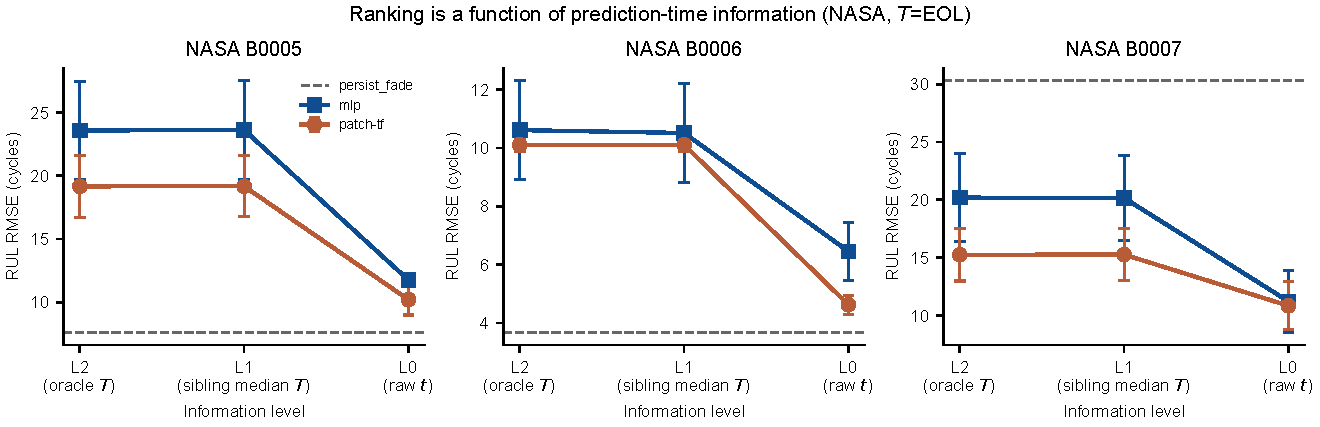
\includegraphics[width=0.98\linewidth]{fig_info_levels.pdf}
\caption{NASA 协议 A 探索阶梯（三种子均值$\pm$标准差）。
虚线为 persist\_fade。L1 与 L2 曲线重合；原始 $t$ 的 L0 是同电芯倒计时。}
\label{fig:ladder}
\end{figure}

\begin{figure}[htbp]
\centering
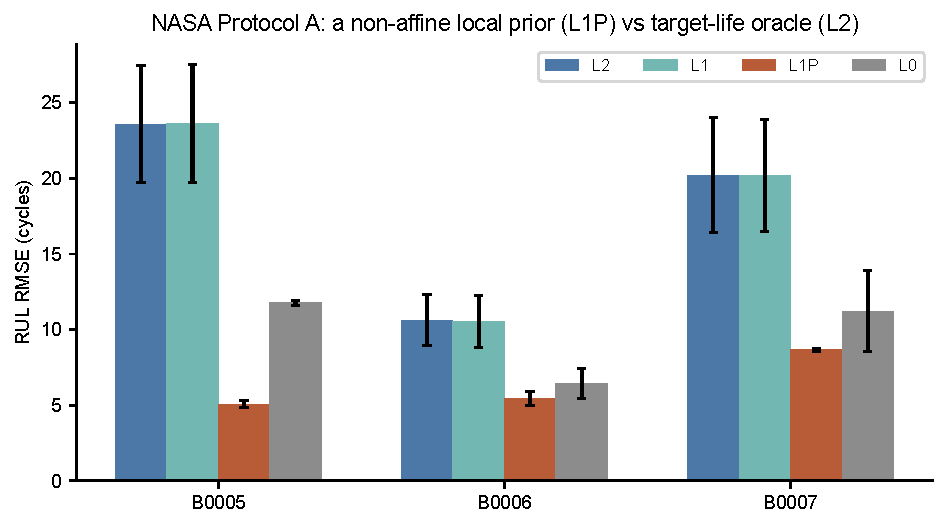
\includegraphics[width=0.98\linewidth]{fig_l1p_nasa.pdf}
\caption{NASA 协议 A 上 L1P 相对 L0/L1/L2（MLP 均值 RMSE）。
三颗电芯上 L1P 均低于 L2（如 B0005：$5.06$ vs.\ $23.58$），对应发现 2。}
\label{fig:l1pnasa}
\end{figure}

\begin{figure}[htbp]
\centering
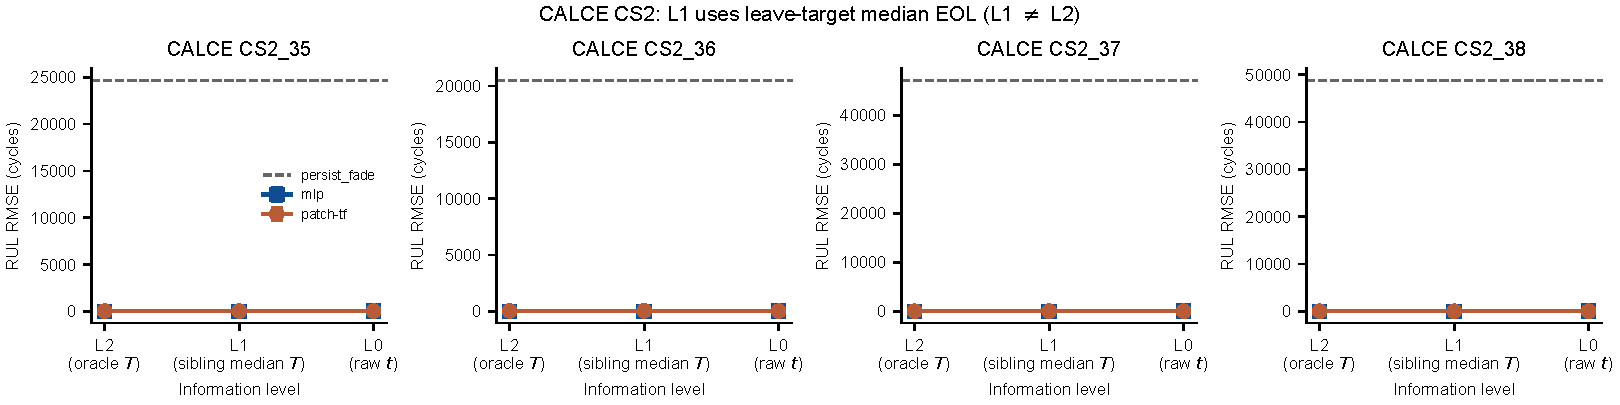
\includegraphics[width=0.98\linewidth]{fig_info_levels_calce.pdf}
\caption{CALCE CS2 探索阶梯（相对 Severson 协议 B 降级）。
MLP 在 CS2\_36--38 上为 L2$\approx$L1 $\ll$ L0。}
\label{fig:laddercalce}
\end{figure}


\subsection{遗留 L2（$T_{\mathrm{record}}$）}
\label{sec:legacy}

本小节为 $T_{\mathrm{record}}$ 下的历史 oracle 基线，非主证据。
表~\ref{tab:l2legacy} 保留原先用记录末循环做 $\mathrm{cycle\_norm}$ 的匹配结果。
这些数字描述的是：已知相对记录终点的进度、且 L1 无法与 L2 分开时的排序。
不删除该表；把它重新标注为寿命定义退化下的 oracle。

\begin{table}[htbp]
\centering
\caption{遗留 L2（$T=T_{\mathrm{record}}$）匹配 RUL RMSE（循环；三种子）。此处 persistence 为未截断时序尾上的 persist\_fade。}
\label{tab:l2legacy}
\begin{tabular}{@{}lcc@{}}
\toprule
模型 & B0005 & B0007 \\
\midrule
persist\_fade & $6.81$ & $30.30$ \\
线性外推 & $7.01$ & $28.10$ \\
MLP & $5.22\pm0.99$ & $\mathbf{5.91\pm1.91}$ \\
Patch-TF & $\mathbf{2.28\pm0.96}$ & $9.67\pm2.95$ \\
\bottomrule
\end{tabular}
\end{table}

去掉 $\mathrm{cycle\_norm}$、其余五通道不变时（L0-drop，同一遗留划分），Patch-TF 与 MLP 落到约 $19$--$22$。
这仍是``头条误差并不来自容量/电压通道本身''的最硬证据。

\subsection{B0007 上 persist\_fade 为何失效}
\label{sec:b0007}

遗留划分上 persist\_fade 在 B0005 为 6.81、在 B0007 为 30.3。
图~\ref{fig:soh}B：B0007 记录末 SOH 约 0.76，EOL 落在最后一循环，晚寿命常出现正增量。
窗口衰减率接近零时，隐含 RUL 会爆炸。
失效因此有两个耦合原因：局部衰减非单调，且目标是\emph{右删失}的——外推到 0.7 等于要求基线虚构一段从未观测到的下降。
L0 合法的递归 persistence 在 B0007 为 15.53、在 B0005 为 6.14（表~\ref{tab:persist}）；persist\_hold$=1$ 因为复制真 $\mathrm{RUL}_{t-1}$，是 oracle。
``L0 下学习模型仍优于 persistence''只可针对 persist\_fade（$30.29$）来写，不可对 persist\_hold 写。

\subsection{修订对照：尺度、匹配、SOH 头、协议 A 区间}
\label{sec:controls}

四项优先对照约束发现 2--3（数据见 \path{outputs/revision_controls/}）。

\paragraph{尺度对照。}
独立匹配的 MLP 重跑（种子 $\{42,43,44\}$；同一协议 A 窗口；非表~\ref{tab:ladder} 训练运行）用于把数值尺度与寿命标签分开。
该重跑中，L1 与 L2 RUL RMSE 相差约 $0.1$ 循环（B0005：$23.62\pm3.17$ vs.\ $23.58\pm3.15$；B0006/B0007 类似），而原始 $t$ 的 L0 在 B0005（$14.92\pm1.48$）与 B0007（$13.58\pm2.76$）更低。
固定尺度 $t/1000$ 即可把 L0 拉向仿射对（B0005：$23.11\pm3.07$）。
L2 均值与表~\ref{tab:ladder} 到小数点后两位一致；种子标准差与 L0 均值因运行不同而不同，故尺度对照数字不得与表~\ref{tab:ladder} 混为同一估计。
该对照表明 L1/L2 行为部分来自数值尺度，而非仅来自寿命常数的语义含义。
点态 $|\hat y^{\mathrm{L1}}-\hat y^{\mathrm{L2}}|$ 均值 $<0.25$、相关 $>0.97$，支持经验尺度稳健性而不声称不变性。

\paragraph{通道支撑。}
NASA 的每个评分测试窗上，L2 通道都高于其训练最大值：$c^{(2)}$ 的测试范围为 $0.85$--$0.99$（B0005）、$0.89$--$0.99$（B0006）、$0.83$--$0.97$（B0007），对应训练上界 $0.85$、$0.88$、$0.83$。
窗口内部值同样如此；常被引用的“$24\%$ 超过训练上界”统计的是测试窗内部的循环，而非窗末值，因而低估了问题。
L1 与 L0 对 $t$ 单调，同样处于支撑外，只是数值范围不同；原始 $t$ 恰好比压缩时钟 $c^{(2)}$ 更易外推，这是尺度效应而非信息效应。
故第~\ref{sec:mechanism} 节把 L2 的失效读作可学习性问题，而不是信息不足。

\paragraph{L1P 匹配距离。}
平均绝对 SOH 匹配距离很小（B0005 $0.0039$；B0006 $0.0307$；B0007 $0.0010$），故 L1P 低于 L2 不是匹配失败伪影。
整条轨迹上，匹配距离与绝对 RUL 误差弱负相关（B0005 $-0.53$；B0006 $-0.59$；B0007 $-0.10$），因为早期窗口同时具有很小的匹配距离和很大的绝对 RUL。
在评分晚寿命窗上符号反转（$0.75$、$0.76$、$0.27$；表~\ref{tab:mechanism}），这才是相关检查：L1P 实际使用时，匹配越差误差越大。

\paragraph{仅 SOH 头 vs.\ 双头（健康默认）。}
表~\ref{tab:sohcontrol} 是支撑默认目标的双头健康检查。
在未归一化消融 $\mathcal{L}_{\mathrm{SOH}}+0.5\,\mathcal{L}_{\mathrm{RUL}}$ 下，SOH RMSE 为 $0.56$--$0.81$，同窗仅 SOH 头可达 $0.017$--$0.031$；$g_{\mathrm{RUL}}/g_{\mathrm{SOH}}$ 达 $64$--$130$，早停由验证 RUL RMSE 驱动，故 SOH 头是欠训练而非不可学。
在\textbf{默认}归一化损失 $\mathcal{L}_{\mathrm{SOH}}+0.5\,\mathcal{L}_{\mathrm{RUL}/T}$ 下，SOH RMSE 恢复到 $0.026$--$0.177$（接近仅 SOH 下限），RUL RMSE 至多变化约 $5$ 循环（B0005 L2：$23.58\to 19.43$），且不改变本文任何信息层级排序——包括 NASA 协议 A 上的 L1P$<$L2 与 Severson 协议 B 上的 L0$\gg$L2。
因此，信息层级结论在 SOH 头已恢复健康的双头配置下依然成立。
完整分层双头表仅保留在附录（表~\ref{tab:soh}）作为多任务诊断，不是 SOH 基准。

\begin{table}[htbp]
\centering
\small
\caption{双头健康检查（NASA 协议 A，L2 通道，三种子，均值$\pm$标准差）。
``消融''为 $\mathcal{L}_{\mathrm{SOH}}+0.5\mathcal{L}_{\mathrm{RUL}}$；``默认（归一）''为 $\mathcal{L}_{\mathrm{SOH}}+0.5\mathcal{L}_{\mathrm{RUL}/T}$；``仅 SOH''以 SOH RMSE 早停。
末列为消融下的 $g_{\mathrm{RUL}}/g_{\mathrm{SOH}}$（前三个 epoch）。
默认 RUL 列为对主文 L2 排序数字的健康模型补充。}
\label{tab:sohcontrol}
\begin{tabular}{@{}lcccccc@{}}
\toprule
电芯 & SOH（消融） & SOH（默认） & 仅 SOH & RUL（消融） & RUL（默认） & $g_{\mathrm{RUL}}/g_{\mathrm{SOH}}$ \\
\midrule
B0005 & $0.706\pm0.184$ & $0.034\pm0.022$ & $0.017\pm0.002$ & $23.58\pm3.85$ & $19.43\pm6.36$ & 124 \\
B0006 & $0.812\pm0.294$ & $0.177\pm0.060$ & $0.031\pm0.005$ & $10.62\pm1.69$ & $15.42\pm7.94$ & 64 \\
B0007 & $0.562\pm0.142$ & $0.026\pm0.014$ & $0.020\pm0.003$ & $20.19\pm3.80$ & $24.51\pm3.89$ & 130 \\
\bottomrule
\end{tabular}
\end{table}

\subsection{SOH 作为辅助对照（附录）}
\label{sec:soh}

附录表~\ref{tab:soh} 报告同窗双头 SOH RMSE。
SOH 不是第二头条任务，也不进入信息层级排序；第~\ref{sec:controls} 节已说明该头的欠训练机制与修复。
双头 SOH 大误差应读作多任务对照失败模式，而非面向 BMS 部署的 SOH 基准；本文没有 RUL 结论依赖该表。
MC-Dropout 仅附录；不作校准声明。共形预测与 PINN 变体不在本文范围。

\section{讨论}
\label{sec:discussion}

当循环通道被赋予不同的寿命常数时，RUL 误差与排序会变。
Severson 协议 B（$n{=}24$）上，MLP 中位 RMSE 由 L0 的 $222.1$ 降至 L2 的 $12.0$，且所评电芯上 L0 均高于 L2（图~\ref{fig:seversonb}）。
该留出目标阶梯是 $\operatorname{Rank}(\cdot\mid\mathcal{I}_t)=f(\mathcal{I}_t)$ 的主支持。

NASA 协议 A 给出更窄、也被机理分析收紧的第二条教训。
即便 SOH 匹配距离很小，L1P 仍可优于 L2（图~\ref{fig:l1pnasa}）：L2 时钟在训练支撑之外被评价，网络压缩晚寿命变化；L1P 则是 SOH 索引的局部平均，停留在匹配邻域内（第~\ref{sec:mechanism} 节）。
这不是“信息越少越好”，而是额外信息在该拟合协议与评分窗上“充分但不可学”，单一 RMSE 列无法揭示这一区别。
协议 B 下反转消失（L1P $30.3$ vs.\ L2 $12.0$），CALCE CS2\_36 上又反过来（L1P $60.69$ vs.\ L2 $2.20$），故正确主张是条件性的。

式~\eqref{eq:affine} 解释协议 A 上 L1 与 L2 为何接近：二者是同一 $t$ 的仿射重标度。
尺度对照支持经验稳健性，但不证明不变性。
协议 B 打破实用上的 L1$\approx$L2，因为单一同胞先验无法在 $T\in[147,1933]$ 上恢复目标特异相对寿命。
协议 A 下，当晚寿命测试窗近似同电芯倒计时时，原始 $t$ 也可优于 L2。
该现象是协议 A 伪影，并不推翻协议 B 的主结果。

这些发现与 Geslin 等关于特征合法性的使用场景观一致~\cite{geslin2023joule,kaufman2012leakage}。
L2 比 L0/L1 信息更多，在回顾性主张下正当；在在线合法主张下，同一 L2 通道信息不一致，应具名为回顾性 oracle。
NASA 协议 A 与 Severson 协议 B 回答不同问题，不应并入同一排名表（第~\ref{sec:decision} 节）。
误差与寿命相关本身也不是 $X_t$ 中存在不合法目标信息的证明。
具名 L0 对照应与学习 L0 并列；persist\_hold 仍是标签 oracle 走步。
NASA+CALCE（$n{=}7$，$p=0.219$）为探索；Severson 协议 B（$p=1.2{\times}10^{-7}$）承担异质寿命应力。

MLP 与 Patch-TF 是匹配预算下的排序仪器。
本文是评价协议，不是 Transformer、PINN 或校准 UQ 主张。

\paragraph{与基准平台的关系。}
BatteryML~\cite{zhang2024batteryml} 与 BatteryLife~\cite{tan2025batterylife} 让数据流水线与模型比较可复现；本文处理的是另一条轴——信息条件的可审计性。
二者互补：数据卡与模型卡可以为每个报告分数附带“信息层级 / 拟合协议 / $T$ 定义 / scaler 来源 / 支撑状态”一行，阶梯可作为其评价外壳的包装层实现，而不改模型。
本文不声称现有平台存在泄漏；我们只指出其报告卡把信息条件留成了隐含项，足以让两个不可比分数并排出现。

\paragraph{局限。}
NASA 与 CALCE 仍为协议 A 诊断。
Severson 协议 B 使用 119 可用电芯中的分层 24 颗应力子集，不是随机总体样本。
除 NASA 循环聚合外，提取缺少完整 in-cycle V/I/T。
全部评分均为完成放电后的循环级任务。

\section{结论}
\label{sec:conclusion}

RUL 基准应把预测时信息写进协议本身。
信息一致评估把通常分散报告的四件事耦合起来：具名信息层级、明确拟合协议、来源与支撑审计、一行一条的可填报告。
在首次 EOL 标签与具名 L0/L1/L1P/L2 通道下，Severson 留出目标评价（$n{=}24$）表明信息层级改变 RUL 误差（L0 $222.1$ vs.\ L2 $12.0$；$p=1.2{\times}10^{-7}$）。
NASA 协议 A 进一步暴露 L1P 优于 L2 的设置特异反转；我们把它追到 oracle 时钟离开训练支撑、而 SOH 索引局部先验仍在匹配邻域内。
此后排行表应一并报告信息层级、拟合协议、$T$ 定义与删失状态、通道支撑与 persist\_fade，而不只写架构名。

\section*{附录. OLS 恒等式检查}
% OLS identity check (appendix only; not a predictive baseline)
\begin{table}[htbp]
\centering
\caption{Appendix OLS identity check on evaluated chronological windows (RUL$>0$).
OLS is an algebraic diagnostic of $\mathrm{RUL}=\max(0,T-t)$, not an out-of-sample predictive baseline: it is fit with an intercept on the same scored windows.
Under that identity, OLS RMSE on raw~$t$ is numerically zero on NASA and CALCE.
$\rho$ is Pearson correlation; $\rho(\mathrm{L1},\mathrm{L2})=1$ because L1 and L2 are affine in~$t$.
L1P is not affine in~$t$.}
\label{tab:clock}
\begin{tabular}{@{}llcccc@{}}
\toprule
Corpus & Cell & $\rho(\mathrm{L1},\mathrm{L2})$ & $\rho(\mathrm{L1P},\mathrm{L2})$ & OLS $t$ & OLS L1P \\
\midrule
nasa & B0005 & 1.000 & -0.703 & 0 & 14.20 \\
nasa & B0006 & 1.000 & -0.598 & 0 & 15.57 \\
nasa & B0007 & 1.000 & -0.824 & 0 & 13.28 \\
calce & CS2\_35 & 1.000 & -0.122 & 0 & 98.18 \\
calce & CS2\_36 & 1.000 & -0.706 & 0 & 101.04 \\
calce & CS2\_37 & 1.000 & -0.654 & 0 & 99.90 \\
calce & CS2\_38 & 1.000 & -0.621 & 0 & 96.29 \\
\bottomrule
\end{tabular}
\end{table}


\section*{附录. 种子级对照与完整 SOH 表}
% auto-generated appendix tables (moved from generated_tables.tex)
\begin{table}[htbp]
\centering
\caption{SOH RMSE (dimensionless; mean$\pm$s.d.\ over three seeds) under the same information ladder.}
\label{tab:soh}
\begin{tabular}{@{}llccc@{}}
\toprule
Model & Cell & L2 & L1 & L0 \\
\midrule
mlp & B0005 & 0.7063$\pm$0.1843 & 0.7007$\pm$0.1826 & 0.3302$\pm$0.0660 \\
mlp & B0006 & 0.8120$\pm$0.2939 & 0.8180$\pm$0.2988 & 0.2879$\pm$0.0462 \\
mlp & B0007 & 0.5625$\pm$0.1420 & 0.5640$\pm$0.1332 & 0.3358$\pm$0.0264 \\
patch-tf & B0005 & 0.3593$\pm$0.0567 & 0.3583$\pm$0.0565 & 0.5132$\pm$0.1256 \\
patch-tf & B0006 & 0.5564$\pm$0.3209 & 0.5548$\pm$0.3199 & 0.4427$\pm$0.0678 \\
patch-tf & B0007 & 0.4028$\pm$0.0108 & 0.4044$\pm$0.0119 & 0.6538$\pm$0.4076 \\
\bottomrule
\end{tabular}
\end{table}

\begin{table}[htbp]
\centering
\caption{Seed-level paired contrasts of RUL RMSE (selected). The experimental unit is the random seed on a fixed cell ($n=3$), not the cell. Wilcoxon $p{=}0.25$ is the smallest two-sided value when all three seeds move in the same direction. Full contrasts are in \texttt{outputs/info\_levels\_v2/stats.json}.}
\label{tab:stats}
\begin{tabular}{@{}llllccc@{}}
\toprule
Contrast & Corpus & Model & Cell & $\Delta$RMSE & Cohen's $d$ & $p$ \\
\midrule
L2-vs-L0 & calce & mlp & CS2\_35 & 30.69 & 13.98 & 0.250 \\
L2-vs-L1 & calce & mlp & CS2\_35 & 0.27 & 0.15 & 0.750 \\
L2-vs-L0 & calce & mlp & CS2\_36 & 38.13 & 21.52 & 0.250 \\
L2-vs-L1 & calce & mlp & CS2\_36 & 0.08 & 0.07 & 0.750 \\
L2-vs-L0 & calce & mlp & CS2\_37 & 42.55 & 22.73 & 0.250 \\
L2-vs-L1 & calce & mlp & CS2\_37 & 0.14 & 0.13 & 0.500 \\
L2-vs-L0 & calce & mlp & CS2\_38 & 34.13 & 10.86 & 0.250 \\
L2-vs-L1 & calce & mlp & CS2\_38 & 0.53 & 0.30 & 0.500 \\
L2-vs-L0 & nasa & mlp & B0005 & -11.81 & -4.33 & 0.250 \\
L2-vs-L1 & nasa & mlp & B0005 & 0.04 & 0.01 & 0.750 \\
L2-vs-L0 & nasa & mlp & B0006 & -4.16 & -3.00 & 0.250 \\
L2-vs-L1 & nasa & mlp & B0006 & -0.10 & -0.06 & 0.250 \\
L2-vs-L0 & nasa & mlp & B0007 & -8.97 & -2.73 & 0.250 \\
L2-vs-L1 & nasa & mlp & B0007 & -0.03 & -0.01 & 1.000 \\
L2-vs-L0 & nasa & patch-tf & B0005 & -8.95 & -4.67 & 0.250 \\
L2-vs-L1 & nasa & patch-tf & B0005 & 0.01 & 0.00 & 1.000 \\
L2-vs-L0 & nasa & patch-tf & B0006 & -5.49 & -19.33 & 0.250 \\
L2-vs-L1 & nasa & patch-tf & B0006 & -0.01 & -0.03 & 0.750 \\
L2-vs-L0 & nasa & patch-tf & B0007 & -4.41 & -2.03 & 0.250 \\
L2-vs-L1 & nasa & patch-tf & B0007 & 0.02 & 0.01 & 0.500 \\
\bottomrule
\end{tabular}
\end{table}



\section*{附录. 报告模板}

\begin{table}[htbp]
\centering
\caption{最低报告行（每个模型 $\times$ 电芯 $\times$ 层级复制一行）。}
\label{tab:template}
\begin{tabular}{@{}p{0.16\linewidth}p{0.18\linewidth}p{0.14\linewidth}p{0.12\linewidth}p{0.16\linewidth}p{0.12\linewidth}@{}}
\toprule
模型 & 层级 & 循环通道 & $W$，$H$ & Scaler & RUL RMSE \\
\midrule
Patch-TF & L0 & 原始 $t$ & 50, 5 & 仅训练期 & \ldots \\
Patch-TF & L1 & $t/T_{\mathrm{med}}$ & 50, 5 & 仅训练期 & \ldots \\
Patch-TF & L2 & $t/T_{\mathrm{target}}$ & 50, 5 & 仅训练期 & \ldots \\
persist\_fade & --- & 仅窗口 SOH & 50, --- & --- & \ldots \\
\bottomrule
\end{tabular}
\end{table}

必报字段：语料、电芯编号、$T$ 定义与是否达到 EOL、是否丢弃 EOL 后窗口、persist\_fade RMSE、拟合协议、通道支撑状态，以及每条学习行的信息层级。
可选：SOH RMSE 作辅助对照；PICP/PINAW 放附录。

\section*{附录. 不确定性（不作校准声明）}
% auto-generated UQ appendix; do not edit by hand
\begin{table}[htbp]
\centering
\caption{Appendix. MC-Dropout 95\% intervals ($n_{\mathrm{MC}}=20$) for Patch-TF RUL on NASA. PICP is empirical coverage of mean$\pm 1.96$ std; PINAW is width normalized by the test RUL range. Not used as a calibration claim.}
\label{tab:uq}
\begin{tabular}{@{}lcccc@{}}
\toprule
Cell & L2 PICP & L2 PINAW & L0 PICP & L0 PINAW \\
\midrule
B0005 & 0.058$\pm$0.025 & 0.599$\pm$0.077 & 0.522$\pm$0.174 & 0.879$\pm$0.167 \\
B0006 & 0.056$\pm$0.048 & 0.709$\pm$0.041 & 0.528$\pm$0.210 & 0.878$\pm$0.265 \\
B0007 & 0.217$\pm$0.075 & 0.607$\pm$0.097 & 0.377$\pm$0.280 & 0.792$\pm$0.165 \\
\bottomrule
\end{tabular}
\end{table}


\section*{声明}
\paragraph{资助。}无。
\paragraph{利益冲突。}无。
\paragraph{数据可得性。}
NASA PCoE B0005--B0007~\cite{saha2007nasa}；CALCE CS2~\cite{he2011calce}；Severson/MATR 批次~\cite{severson2019nature}。
复现脚本与采用实验结果：\path{scripts/run_info_levels_v2.py}，\path{scripts/run_revision_controls.py}，\path{scripts/run_l1p_mechanism.py}，\path{experiments/info_consistent/}，\path{outputs/info_levels_v2/}，\path{outputs/info_levels_severson_loco/}，\path{outputs/revision_controls/}，\path{outputs/l1p_mechanism/}。
代码与采用实验结果见 \url{https://github.com/Jiang-52/info-consistent-battery-rul}（详见 \path{CODE_AVAILABILITY.md}）。Zenodo DOI 将在首次存档后补入。

\begin{thebibliography}{99}

%% ---- foundational corpora / protocol anchors (pre-2025 minority) ----
\bibitem{saha2007nasa}
B.~Saha, K.~Goebel,
Battery Data Set,
NASA Ames Prognostics Data Repository,
Moffett Field, CA (2007).

\bibitem{saha2009compare}
B.~Saha, K.~Goebel, J.~Christophersen,
Comparison of prognostic algorithms for estimating remaining useful life of batteries,
Trans.\ Inst.\ Meas.\ Control 31~(3--4) (2009) 293--308.

\bibitem{he2011calce}
W.~He, N.~Williard, M.~Osterman, M.~Pecht,
Prognostics of lithium-ion batteries based on Dempster--Shafer theory and the Bayesian Monte Carlo method,
J.\ Power Sources 196~(23) (2011) 10314--10321.

\bibitem{kaufman2012leakage}
S.~Kaufman, S.~Rosset, C.~Perlich, O.~Stitelman,
Leakage in data mining: Formulation, detection, and avoidance,
ACM Trans.\ Knowl.\ Discov.\ Data 6~(4) (2012) 1--21.

\bibitem{gal2016}
Y.~Gal, Z.~Ghahramani,
Dropout as a Bayesian approximation: representing model uncertainty in deep learning,
in: Proc.\ 33rd Int.\ Conf.\ Mach.\ Learn., PMLR 48 (2016) 1050--1059.

\bibitem{vaswani2017}
A.~Vaswani, N.~Shazeer, N.~Parmar, J.~Uszkoreit, L.~Jones, A.N.~Gomez, L.~Kaiser, I.~Polosukhin,
Attention is all you need,
in: Adv.\ Neural Inf.\ Process.\ Syst.\ 30 (2017) 5998--6008.

\bibitem{birkl2017}
C.R.~Birkl, M.R.~Roberts, E.~McTurk, P.G.~Bruce, D.A.~Howey,
Degradation diagnostics for lithium ion cells,
J.\ Power Sources 341 (2017) 373--386.

\bibitem{xiong2018soh}
R.~Xiong, L.~Li, J.~Tian,
Towards a smarter battery management system: a critical review on battery state of health monitoring methods,
J.\ Power Sources 405 (2018) 18--29.

\bibitem{lipu2018}
M.S.H.~Lipu, M.A.~Hannan, A.~Hussain, M.M.~Hoque, P.J.~Ker, S.M.A.~Saad, A.~Ayob,
A review of state of health and remaining useful life estimation methods for lithium-ion battery in electric vehicles: challenges and recommendations,
J.\ Clean.\ Prod.\ 205 (2018) 115--133.

\bibitem{hu2019rser}
X.~Hu, F.~Feng, K.~Liu, L.~Zhang, J.~Xie, B.~Liu,
State estimation for advanced battery management: key challenges and future trends,
Renew.\ Sustain.\ Energy Rev.\ 114 (2019) 109334.

\bibitem{severson2019nature}
K.A.~Severson, P.M.~Attia, N.~Jin, N.~Perkins, B.~Jiang, Z.~Yang, M.H.~Chen, M.~Aykol, P.K.~Herring, D.~Fraggedakis, M.Z.~Bazant, S.J.~Harris, W.C.~Chueh, R.D.~Braatz,
Data-driven prediction of battery cycle life before capacity degradation,
Nat.\ Energy 4 (2019) 383--391.

\bibitem{roman2021}
D.~Roman, S.~Saxena, V.~Robu, M.~Pecht, D.~Flynn,
Machine learning pipeline for battery state-of-health estimation,
Nat.\ Mach.\ Intell.\ 3 (2021) 447--456.

\bibitem{sulzer2021joule}
V.~Sulzer, P.~Mohtat, A.~Aitio, S.~Lee, Y.T.~Yeh, F.~Steinbacher, M.U.~Khan, J.W.~Lee, J.B.~Siegel, A.G.~Stefanopoulou, D.A.~Howey,
The challenge and opportunity of battery lifetime prediction from field data,
Joule 5 (2021) 1934--1955.

\bibitem{geslin2023joule}
A.~Geslin, B.~van Vlijmen, X.~Cui, A.~Bhargava, P.A.~Asinger, R.D.~Braatz, W.C.~Chueh,
Selecting the appropriate features in battery lifetime predictions,
Joule 7 (2023) 1956--1965.

\bibitem{kapoor2023leakage}
S.~Kapoor, A.~Narayanan,
Leakage and the reproducibility crisis in machine-learning-based science,
Patterns 4~(9) (2023) 100804.

\bibitem{nie2023patchtst}
Y.~Nie, N.H.~Nguyen, P.~Sinthong, J.~Kalagnanam,
A time series is worth 64 words: long-term forecasting with transformers,
in: Int.\ Conf.\ Learn.\ Represent.\ (2023).

\bibitem{rosenblatt2024}
M.~Rosenblatt, L.~Tejavibulya, R.~Jiang, S.M.~Noble, D.~Scheinost,
Data leakage inflates prediction performance in connectome-based machine learning models,
Nat.\ Commun.\ 15 (2024) 1829.

\bibitem{zhang2024batteryml}
H.~Zhang, X.~Gui, S.~Zheng, Z.~Lu, Y.~Li, J.~Bian,
BatteryML: An open-source platform for machine learning on battery degradation,
in: Int.\ Conf.\ Learn.\ Represent.\ (2024).

\bibitem{li2024lifetime}
T.~Li, Z.~Zhou, A.~Thelen, D.A.~Howey, C.~Hu,
Predicting battery lifetime under varying usage conditions from early aging data,
Cell Rep.\ Phys.\ Sci.\ 5~(4) (2024) 101891.

%% ---- 2025--2026 majority ----
\bibitem{wang2024gce}
S.~Wang, R.~Zhou, Y.~Ren, M.~Jiao, H.~Liu, C.~Lian,
Advanced data-driven techniques in AI for predicting lithium-ion battery remaining useful life: a comprehensive review,
Green Chem.\ Eng.\ 6~(2) (2025) 139--153.

\bibitem{zhang2025batlinet}
H.~Zhang, Y.~Li, S.~Zheng, Z.~Lu, X.~Gui, W.~Xu, J.~Bian,
Battery lifetime prediction across diverse ageing conditions with inter-cell deep learning,
Nat.\ Mach.\ Intell.\ 7 (2025) 270--277.

\bibitem{tan2025batterylife}
R.~Tan, W.~Hong, J.~Tang, X.~Lu, R.~Ma, X.~Zheng, J.~Li, J.~Huang, T.-Y.~Zhang,
BatteryLife: A comprehensive dataset and benchmark for battery life prediction,
arXiv:2502.18807 (2025).

\bibitem{madani2025groupkfold}
S.S.~Madani, M.~H\'{e}bert, L.~Boulon, A.~Lupien-B\'{e}dard, F.~Allard,
Comparative analysis of ML and DL models for data-driven SOH estimation of LIBs under diverse temperature and load conditions,
Batteries 11~(11) (2025) 393.

\bibitem{xu2025meas}
Z.~Xu, J.~Mao, Y.~Han, H.~Yuan,
A comprehensive review of lithium-ion battery remaining useful life prediction: methodologies, datasets, performance metrics, and future perspectives,
Meas.\ Sci.\ Technol.\ 36~(8) (2025) 082001.

\bibitem{yang2025batteries}
Y.~Yang, S.~Wang, Y.~Zhou, C.~Fernandez,
A critical review of AI-based battery remaining useful life prediction for energy storage systems,
Batteries 11~(10) (2025) 376.

\bibitem{deng2025piml}
Y.~Deng, X.~Le, T.T.~Nguyen, C.~Gogu,
A generic physics-informed machine learning framework for battery remaining useful life prediction using small early-stage lifecycle data,
Appl.\ Energy 384 (2025) 125314.

\bibitem{oyewole2025uq}
I.~Oyewole, W.~Hassanieh, M.~Chelbi, A.~Chehade,
Uncertainty-aware deep learning with physics-informed bayesian sampling for lithium-ion battery prognostics,
Appl.\ Energy 402 (2025) 126880.

\bibitem{aliakbari2025fusedr}
S.~Aliakbari, M.~Masih-Tehrani,
FuseDR-Net: a fusion-based network for battery remaining useful life prediction using causally decomposed health indicators,
Energy Convers.\ Manag.\ X 28 (2025) 101341.

\bibitem{ge2025koopman}
X.~Ge, Y.~Jiang, B.~Xu,
Deep Koopman operator-based remaining useful life prediction of Lithium-ion batteries under multi-condition scenarios,
J.\ Energy Storage 119 (2025) 116369.

\bibitem{li2025adapt}
J.~Li, Z.~Wang, D.~Tian, Z.~Sun, Y.~Niu,
A novel RUL prediction framework based on the adaptability feature perception fusion model method,
J.\ Energy Storage 119 (2025) 116322.

\bibitem{huang2025rulmamba}
J.~Huang, L.~Liu, H.~Zhao, T.~Li, B.~Li,
RUL-Mamba: Mamba-based remaining useful life prediction for lithium-ion batteries,
J.\ Energy Storage 120 (2025) 116376.

\bibitem{tian2025energy}
A.~Tian, H.~Yu, Z.~Hu, Y.~Wang, T.~Wu, J.~Jiang,
A novel remaining useful life prediction method based on CNN-Attention combined with SMA-GPR,
Energy 321 (2025) 135233.

\bibitem{yi2025jps}
X.~Yi, J.~Xiao, G.~Lei, X.-H.~Hu, Z.~Feng,
A lithium-ion battery remaining useful life prediction model based on multilayer perceptron expert networks and temporal feature composition,
J.\ Power Sources 659 (2025) 238371.

\bibitem{wang2025jes}
K.~Wang, J.~Wang, Z.~Wang, H.~Li,
An enhanced deep learning framework for state of health and remaining useful life prediction of lithium-ion battery based on discharge fragments,
J.\ Energy Storage 107 (2025) 114952.

\bibitem{ali2026loco}
B.~Ali, I.~Matloob, N.~Alkhalifa, A.K.~Alkhalifa, N.~Asim, S.~Kanwal, S.~Inam,
Deep learning-based RUL and SOH prediction of lithium-ion batteries using LOCO,
Sci.\ Rep.\ 16 (2026) 27853.

\bibitem{barua2026predictor}
A.~Barua, J.M.~Collins, M.R.~Islam, S.~Barua,
Predictor structure modulates validation inflation and cell-transfer reliability in battery state-of-health estimation,
Batteries 12~(9) (2026) 342.

\bibitem{sun2026sgdits}
Y.~Sun, F.~Gao,
SG-DiTs: A physics-informed diffusion-transformer hybrid framework for reliable battery RUL prediction,
J.\ Energy Storage 152 (2026) 120479.

\bibitem{fan2026meas}
Y.~Fan, Z.~Xu, H.~Zhu, Y.~Yu,
Physics-informed signal decomposition and data-driven RUL estimation for lithium-ion batteries,
Meas.\ Sci.\ Technol.\ 37~(18) (2026) 186103.

\bibitem{li2026dpmamba}
X.~Li, H.~Zhang,
DpMamba: a dual-path state space model for reliable remaining useful life prediction of lithium-ion batteries,
Meas.\ Sci.\ Technol.\ 37~(34) (2026) 346105.

\end{thebibliography}


\end{document}